\section{Оборудование}
\begin{figure}[ht!]
    \centering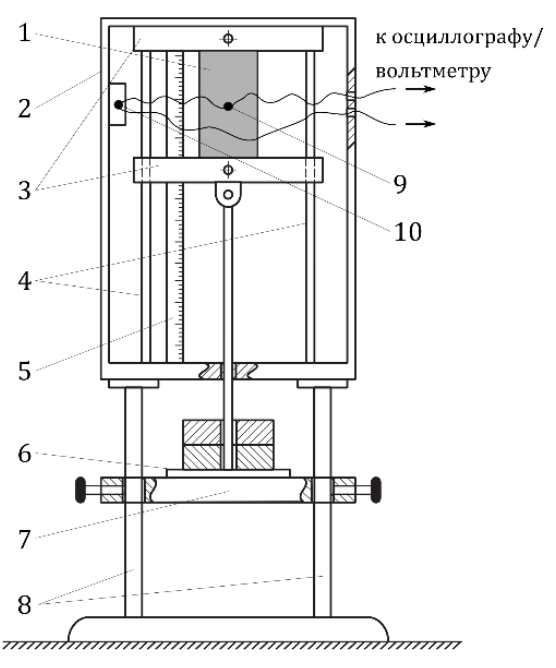
\includegraphics[width=0.8\linewidth]{img/kal.png}
\end{figure}

Схема экспериментальной установки изображена на рисунке. Исследуемый образец 1
(плоская резиновая полоса) расположен внутри закрытого кожуха 2 и закреплён в зажимах 3. 
Верхний зажим неподвижен, а нижний может свободно перемещаться вдоль вертикальных
направляющих 4. Положение нижнего зажима измеряется линейкой 5. К нижнему зажиму подвешена
платформа 6, на которой могут размещаться грузы. Растяжение образца может быть ограничено
положением упора 7, фиксируемого винтами на стойке 8.

Внутри резиновой полосы (в её центре) вшит один из спаев термопары 9 (рабочий спай).
Второй (компенсирующий) спай 10 находится внутри кожуха вблизи стенки. Выводы термопар
подключаются к микровольтметру, либо через усилитель к цифровому осциллографу.
Характеристики термопары и усилителя указаны на установке.

Изменение температуры резины $\Delta T$ составляет всего несколько десятых долей градуса.
Поэтому в работе важно максимально
точно обеспечить равенство начальных температур рабочего и компенсирующего спаев.
Чтобы лучше выровнять начальные температуры, образец вместе
с термопарами помещён в закрытый кожух, стенки которого для лучшей изоляции покрыты
алюминиевой фольгой. При работе необходимо избегать перепадов температур
как внутри кожуха, так и вблизи него: в частности, не
следует направлять на кожух настольную лампу (для подсветки можно использовать
светодиодный фонарик); не следует без необходимости трогать кожух руками; также стоит
убедиться, что в помещении отсутствуют значимые
перепады температур (закрыть окна и т.п.).

Измерение термического эффекта при адиабатическом растяжении можно
провести двумя способами. Можно быстро растянуть резину и непосредственно измерить
возникающий температурный скачок. Либо можно
растягивать резину медленнее, а затем экстраполировать кривую зависимости
температуры от времени к начальному моменту. Оба способа обладают своими недостатками:
при быстром растяжении возможно возникновение необратимых явлений, а при использовании
же второго способа неизбежна ошибка экстраполяции, величину которой трудно оценить.
